\documentclass[tikz,border=2pt]{standalone}
\usepackage{amsmath,amssymb}
\usepackage{tikz}
\usetikzlibrary{arrows.meta}

\begin{document}
% {1/n : n>=1} has a maximum (1) but no minimum: the infimum 0 is not in the set.
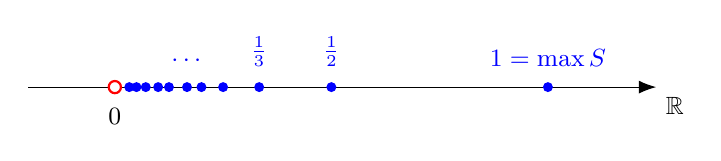
\begin{tikzpicture}[x=5.5cm, every node/.style={font=\small}]
	\draw[-{Latex[length=2.2mm]}] (-0.2,0) -- (1.25,0) node[below right] {$\mathbb{R}$};
	\foreach \n in {1,2,3,4,5,6,8,10,14,20,30} {\fill[blue] ({1/\n},0) circle (1.8pt);}
	\draw[red, thick, fill=white] (0,0) circle (2.2pt);
	\node[below=4pt] at (0,0) {$0$};
	\node[blue, above=4pt] at (1,0) {$1=\max S$};
	\node[blue, above=4pt] at (0.5,0) {$\tfrac12$};
	\node[blue, above=4pt] at (0.333,0) {$\tfrac13$};
	\node[blue, above=4pt, font=\small] at (0.17,0) {$\cdots$};
\end{tikzpicture}
\end{document}
